% ---------
%  Compile with "./build.sh"
% --------

\documentclass[10pt]{article}
\usepackage{amsmath}
\usepackage[margin=1in]{geometry}
\usepackage{import}
\usepackage{amssymb}
\usepackage{float}
\usepackage{listings}
\usepackage{graphicx}
\usepackage{cite}
\usepackage[ruled,vlined]{algorithm2e}
\usepackage[utf8]{inputenc}		% Allow some non-ASCII Unicode in source

\begin{document}
\section{Course Project}

Taxonomic identification and phylogenetic profiling software TIPP
\cite{nguyen_tipp_2014} requires solving a phylogenetic placement problem in order to
insert a new alignment into a tree. Currently, software such as pplacer
\cite{matsen_pplacer_2010} is an accurate, maximum likelihood phylogenetic placement
method. However, pplacer does not scale to problems larger than 1,000
sequences. Therefore, alternative phylogenetic placement methods, such
as APPLES \cite{balaban_apples_2020}, were developed for solving phylogenetic placement.
While APPLES has been tested to run on 200,000 sequences, the accuracy
of the method for smaller problems is typically worse than pplacer. This
course project aims to improve phylogenetic placement software already
available in two different approaches. The first proposed approach runs
pplacer in a divide-and-conquer scheme to determine the optimal
placement of the query sequence. The second approach, however, uses
APPLES to identity the most probable region for a query sequence. Once
this region is identified, pplacer is used on some collection of clades
around this region of the tree in order to determine a more accurate
placement.

\subsection{Approach 1}

Approach 1 aims to solve the placement problem by using a
divide-and-conquer approach, using pplacer to solve the smaller
phylogenetic placement problems. The first step of this approach is to
divide the backbone tree into problems small enough that pplacer can
readily be used. The software will divide the backbone into disjoint
subtrees with fewer than 1000 sequences each. This will be done
similarly to the first step of PASTA described in \cite{PASTA}, using
centroid decomposition. A centroid decomposition approach is used to
determine subtrees smaller than some prescribed size, such as 1000
sequences. The centroid decomposition determines a centroid edge in the
tree that partitions the tree into two halves of roughly equal size.
Each subtree is then recursively subdivided using this same approach,
until each subtree has no more sequences that the prescribed limit. We
will start with the maximum size of the subtrees at 1000 sequences. We
will also consider if it may improve the accuracy to have smaller trees,
such as 500 sequences, though based on the placement accuracy by
reference tree size in the comparison to APPLES in \cite{balaban_apples_2020}, we expect
that accuracy will be higher for larger reference trees. After
decomposing the tree via centroid decomposition, the query sequence will
be placed into each of the subtrees generated. Pplacer will run
independently on each of the subtrees from this centroid decomposition.
Since each subproblem is independent of the other subproblems, this step
in the algorithm is embarassingly parallel.

After determining the placement on each subtree, the placement of the
query sequence on the subtree is used as the placement of the query
sequence into the backbone tree. Each backbone tree returned from this
method can then be compared, and the one with the best score is taken as
the output from the algorithm. Each tree is scored using RAxML in
fixed-tree mode, allowing us to compare the maximum likelihood score of
each of the placement trees. Based on the location of the best score on
the best subtree, the algorithm returns the corresponding location on
the original backbone tree. Pseudocode for approach 1 is shown below in
algorithm \ref{alg:approach1}.
The pipeline for approach 1 is also shown below in figure \ref{fig:approach1-pipeline}.

\begin{figure}[h]
\centering
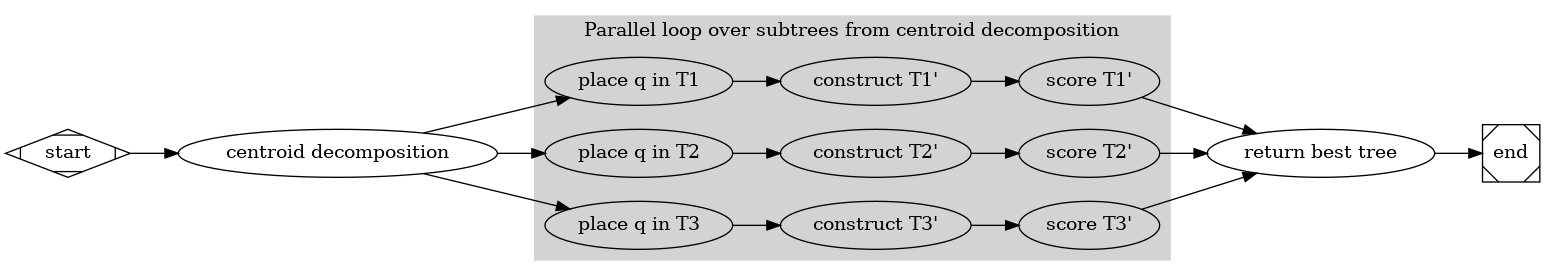
\includegraphics[width=\textwidth]{Figs/pipeline1.png}
\label{fig:approach1-pipeline}
\caption{Pipeline for approach 1. Placements inside the parallel region over
the sub trees identified by the centroid decomposition are evaluated
using pplacer.
The overall placement on the backbone trees is scored by the log-likelihood
from running raxml-ng in fixed tree, fixed parameter mode.
}
\end{figure}

\subsection{Approach 2}

Approach 2 aims to combine the scalability of APPLES with the accuracy
empirically seen for pplacer on smaller subtrees. Initially, APPLES is
run on the query sequence and the entire backbone tree. The placement
returned from APPLES is then used to identify a collection of
(relatively) small clades containing this placement. Each clade is
chosen to be smaller than some prescribed size, such as 1000 sequences.
Since there is not a single unique clade satisfying this property, some
(random) collection of clades is considered. If time permits, a more
sophisticated method for determining clades in the backbone tree
containing the query sequence may be considered. Psuedocode for
generating a single (random) clade are shown below in algorithm
\ref{alg:clade-grabber}. Balaban et al.~observed that, for the RNASim-VS
data set, the delta errors in APPLES's placement are likely to be
relatively small. This indicates that the placement of the query
sequence into the tree may be quite close to the true placement, meaning
that only a small refinment is needed to produce the correct result.
Pplacer is used on each of the clades identified in the previous step.
Note that, similar to the previous approach, the placement and scoring
on each clade is completely independent of the other clades. This makes
this portion of the algorithm embarrasingly parallel. As in the other
approaches, the final result is the placement of the query sequence in
the original backbone tree based on its subtree placement. The placement
that minimizes the maximum likelihood scores, as computed by RAxML in
fixed tree mode, is then chosen as the placement returned by the
algorithm. Note also that the original placement, as determine by
APPLES, is also included in this consideration. Pseudocode for approach
2 is shown below in algorithm \ref{alg:approach2}.
The pipeline for approach 2 is also shown below in figure \ref{fig:approach2-pipeline}.

\begin{figure}[h]
\centering
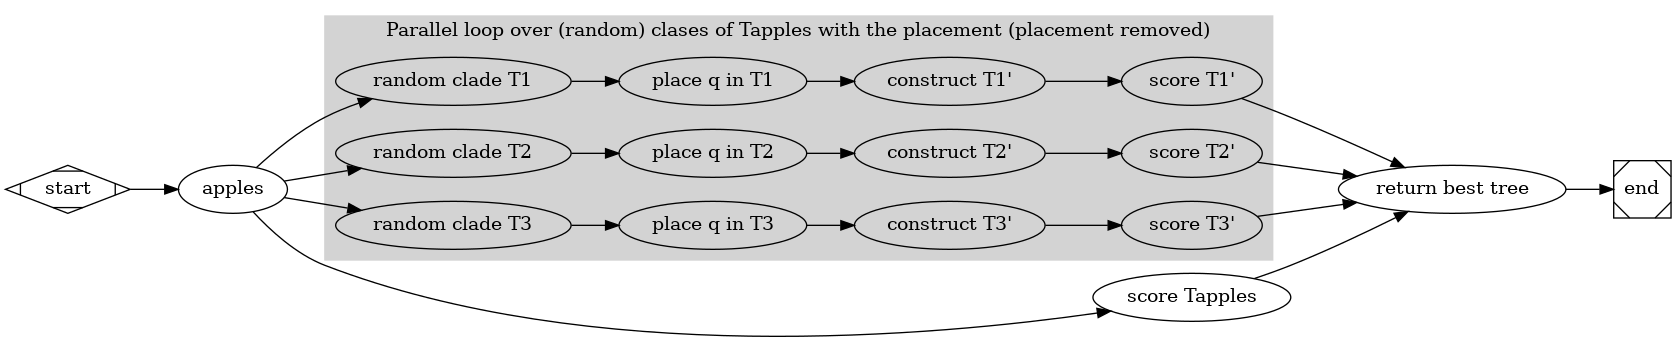
\includegraphics[width=\textwidth]{Figs/pipeline2.png}
\label{fig:approach2-pipeline}
\caption{Pipeline for approach 2.
APPLES is initially used to find a tentative placement for the query sequence.
Random clades about the query placement are generated
up to some provided fixed size.
The query sequence is then placed in each clade
using pplacer.
The overall placement on the backbone trees is scored by the log-likelihood
from running raxml-ng in fixed tree, fixed parameter mode.
}
\end{figure}

\section{Data}

\subsection{Testing Data}

We will use the 1000M1 dataset from \cite{sate}. This includes 20 replicate
datasets.

\subsection{Benchmarking Data}

For simulated data, we will use the same datasets as APPLES used from
\cite{guo}, and use the RNASim-VS sets. These sets are of size 500, 1000,
5000, 10,000, 50,000, 100,000 and 200,000. For each of the sizes, there
are a total of 5 replicates. The 200,000 sequence data set, however,
only has a single replicate.

\section{Assessment}

\subsection{Asessment Criteria}

We will be comparing to both pplacer and APPLES for accuracy and
runtime. For small backbone trees (less than 1000 sequences), our
approach will equivalent to pplacer, so the accuracy at that point
should be equal with no meaningful increase in runtime. For larger
trees, we will look at the error rate relative to APPLES and at how the
implementation scales. To calculate the error, we will use the same
delta error calculation as APPLES to compare the sets of bipartions for
the tree with the placement from our system and the bipartion from the
tree with the correct placement. In concrete terms, delta error is
defined as
\begin{align*}
\Delta e(P) = \vert B(T^*) \backslash B(P) \vert - \vert B(T^* \upharpoonright_{\mathcal L}) \backslash B(T)\vert,
\end{align*}
where $\mathcal L$ denotes the leafset, \(P\) denotes the tree
after placement, $T^*$ denotes the true tree on
$\mathcal L \cup \{q\}$, $T^* \upharpoonright_{\mathcal L}$ denotes
the true tree restricted to $\mathcal L$, and $B(\cdot)$ denotes the
bipartition set of a tree \cite{balaban_apples_2020}.

Similar to Balaban and coworkers \cite{balaban_apples_2020}, we plan to consider a
leave-one-out strategy in testing and evaluating the 1000M1 and
RNASim-VS datasets. The leave-one-out strategy starts with the true
tree, \(T\), and identifies a random leaf node \(q\) from the tree. This
leaf node is removed and then added back into the tree \(T\) using the
placement software. This process is repeated 200 times to generate a
distribution of errors produced by the placement software.

\subsection{Analysis Hardware}

We will perform the analysis on NCSA's Blue Waters. Each Blue Waters XE
node has 16 cores. As neither APPLES nor pplacer has GPU capabilities,
we will use the XE nodes instead of the XK nodes. Development and small
testing will be conducted on the campuscluster or monza, a 12 core
workstation.

\subsection{Software}

For comparison and steps of the implementation, we will be using both
APPLES and pplacer. For the implementation, we will also use RAxML
\cite{raxml}.

We will use APPLES version 1.3.0, which requires Python 3. The code can
be found at:\newline https://github.com/balabanmetin/apples. We will
only be running APPLES with alignment, as pplacer requires an alignment.

The command for APPLES will be:

\begin{verbatim}
python3 ~/apples/run_apples.py -t backbone.nwk -s aln_dna.fa -q query.fa -T 16 -o apples.jplace
\end{verbatim}

We will use pplacer version v1.1.alpha19-0-g807f6f3. The binary files
can be found at:\newline
https://github.com/matsen/pplacer/releases/tag/v1.1.alpha19.

The command for pplacer will be:

\begin{verbatim}
pplacer -m GTR -s RAxML_info.REF -t backbone.nwk -o query.jplace aln_dna.fa -j 1
\end{verbatim}

We will use the sequential RAxML version 8.2.12. Parallelism with RAxML
will be done through calling RAxML in a multithreaded section. This will
be used to compare different pplacer outputs in both approaches. The
maximum likelihood score returned from RAxML in fixed tree mode is used
as the score for the two approaches. The command for RAxML-NG will be:

\begin{verbatim}
./raxml-ng --evaluate --model GTR+G --tree test.tree
\end{verbatim}

\subsection{Approach 1 Pseudocode}

\begin{algorithm}[H]
\SetKwFor{ParallelFor}{parallel for}{do}{endfor}
\SetAlgoLined
\KwResult{$T'$, tree T with query sequence $q$ added}
\KwIn{Tree $T$ on $N$ sequences, the MSA of $N+1$ sequences, and query sequence $q$}
 // $\operatorname{centroidDecomposition}$ decomposes a tree into roughly equal size, disjoint parts until the trees are no larger than the prescribed size.\;
 // $\operatorname{modifyTree}$ adds sequence to a tree based on the sequence's location in the a subtree with the sequence added\;
 $\{T_1,\dots,T_n\} \leftarrow \operatorname{centroidDecomposition}(T,1000)$\;
 $\{S_1, \dots, S_n\} \leftarrow 0$ // Score for each tree\;
 \ParallelFor{$i=1,\dots,n$}{
  // Place query sequence $q$ into the subtree\;
  $T'_i \leftarrow \operatorname{pplacer}(T_i, q)$\;
  // Add the location of the query sequence $q$ to a copy of $T$\;
  $T_{q_{i}} \leftarrow \operatorname{modifyTree}(T, T'_i, q)$\;
  // $\operatorname{RAxMLScorer}$ runs RAxML in fixed tree mode.\;
  // The output score is the maximum likelihood found on the tree.\;
  $S_i \leftarrow \operatorname{RAxMLScorer}( T_{q_{i}})$\;
 }
 // Do a maxLoc reduction for the tree\;
 $bestTreeIndex \leftarrow \operatorname{argmax}_{i} (S_1,\dots,S_n)$\;
 return $T'_{q_{bestTreeIndex}}$\;
 \caption{divide-and-conquer pplacer}
 \label{alg:approach1}
\end{algorithm}

\subsection{Approach 2 Pseudocode}

\begin{algorithm}[H]
\SetKwFor{ParallelFor}{parallel for}{do}{endfor}
\SetAlgoLined
\KwResult{$T'$, tree T with query sequence $q$ added}
\KwIn{Tree $T$ on $N$ sequences, the MSA of $N+1$ sequences, query sequence $q$,
and the number of clades considered, $N_{clades}$.
}
 // $\operatorname{modifyTree}$ adds sequence to a tree based on the sequence's location in the a subtree with the sequence added\;
 // $\operatorname{getRegion}$ finds a subtree containing the sequence with a maximum number of sequences\;
  // Run APPLES\;
  $T'_{APPLES} \leftarrow \operatorname{APPLES}(T, q)$\;
  // It could be the case that APPLES produces the best score\;
  $S_{apples} \leftarrow \operatorname{RAxMLScorer}( T'_{apples})$\;
  $\{S_1, \dots, S_{N_{clades}}\} \leftarrow 0$ // Score for each clade\;
  \ParallelFor{$i=1,\dots, N_{clades}$}{
    // Identify (random) region of T where q was placed with fewer than 1000 sequences\;
    $T_{i} \leftarrow \operatorname{getRegion}(T'_{APPLES}, q, 1000)$\;
    // Run pplacer on the area of T around the placement of q\;
    $T'_{pplacer} \leftarrow \operatorname{pplacer}(T_{i})$\;
  // Add the location of the query sequence $q$ to a copy of $T$\;
  $T_{q_{i}} \leftarrow \operatorname{modifyTree}(T, T_{i}, q)$\;
  // $\operatorname{RAxMLScorer}$ runs RAxML in fixed tree mode.\;
  // The output score is the maximum likelihood found on the tree.\;
  $S_i \leftarrow \operatorname{RAxMLScorer}( T_{q_{i}})$\;
  }
 // Do a maxLoc reduction for the tree\;
 $bestTreeIndex \leftarrow \operatorname{argmax}_{i} (S_{apples},S_1,\dots,S_n)$\;
 return $T'_{q_{bestTreeIndex}}$\;
\caption{APPLES with pplacer}
 \label{alg:approach2}
\end{algorithm}

\begin{figure}[H]
\centering
\begin{lstlisting}[language=python]
# code from Vlad Smirnov. Generates a clade of a maximum size given a leaf node.
def getRegion(leaf, size):
    taxons = [leaf.taxon.label]
    node = leaf
    while len(taxons) < size:
        shuffledSiblingNodes = node.sibling_nodes().copy()
        for bro in shuffledSiblingNodes:
            taxons.extend(collectSubtreeTaxa(bro, size - len(taxons)))
            if len(taxons) >= size:
                return taxons
        node = node.parent_node
    return taxons
def collectSubtreeTaxa(node, numTaxa):
    if node.is_leaf():
        return [node.taxon.label]
    taxons = []
    shuffledChildNodes = node.child_nodes().copy()
    random.shuffle(shuffledChildNodes)
    for child in shuffledChildNodes:
        taxons.extend(collectSubtreeTaxa(child, numTaxa - len(taxons)))
        if len(taxons) >= numTaxa:
            return taxons
    return taxons
\end{lstlisting}
\label{alg:clade-grabber}
\end{figure}

\bibliographystyle{plain}
\bibliography{cs581-project}

\end{document}

